%%%%%%%%%%%%%%%%%%%%%%%%%%%%%%%%%%%%%%%%%
% Document Author: Plinio H. Vargas
% Course: CS-532, Spring 2016 at Old Dominion University
%
% Structured General Purpose Assignment
% LaTeX Template
%
% This template has been downloaded from:
% http://www.latextemplates.com
%
% Original template author:
% Ted Pavlic (http://www.tedpavlic.com)
%
% Note:
% The \lipsum[#] commands throughout this template generate dummy text
% to fill the template out. These commands should all be removed when 
% writing assignment content.
%
%%%%%%%%%%%%%%%%%%%%%%%%%%%%%%%%%%%%%%%%%
%----------------------------------------------------------------------------------------
%	PACKAGES AND OTHER DOCUMENT CONFIGURATIONS
%----------------------------------------------------------------------------------------

\documentclass{article}

\usepackage{fancyhdr} % Required for custom headers
\usepackage{lastpage} % Required to determine the last page for the footer
\usepackage{extramarks} % Required for headers and footers
\usepackage{listings}
\usepackage{graphicx} % Required to insert images
\usepackage{lipsum} % Used for inserting dummy 'Lorem ipsum' text into the template
\usepackage[bookmarks,bookmarksopen,bookmarksdepth=2]{hyperref} % for bookmarks
\usepackage{enumerate}
\usepackage{csquotes} % for quoting things
\usepackage{multirow}
\usepackage{amsmath}
\usepackage{caption}
\usepackage{navigator}%\usepackage{caption}
\usepackage[shortlabels]{enumitem}
\usepackage{enumitem}
\usepackage{lmodern}
\usepackage[utf8]{inputenc}
%\usepackage[table]{xcolor}% http://ctan.org/pkg/xcolo
\usepackage[dvipsnames]{xcolor}
\usepackage{longtable}
\usepackage{textcomp}
\usepackage{url}
\usepackage{import}
\usepackage{float}
\usepackage{dashrule} % for dashline
\usepackage{keystroke}
\usepackage{amssymb}
\usepackage{booktabs}

\lstdefinestyle{numbers}
{ frame=tb,
  language=python,
  aboveskip=3mm,
  belowskip=3mm,
  showstringspaces=false,
  columns=flexible,
  basicstyle={\small\ttfamily},
  numbers=left,
  numberstyle=\tiny\color{gray},
  keywordstyle=\color{blue},
  commentstyle=\color{OliveGreen},
  stringstyle=\color{purple},
  breaklines=true,
  breakatwhitespace=true,
  tabsize=3
}

\lstdefinestyle{nonumbers}
{ frame=shadowbox,
  language=python,
  aboveskip=3mm,
  belowskip=3mm,
  showstringspaces=false,
  columns=flexible,
  basicstyle={\small\ttfamily},
  numbers=none,
  numberstyle=\tiny\color{gray},
  keywordstyle=\color{blue},
  commentstyle=\color{OliveGreen},
  stringstyle=\color{purple},
  breaklines=true,
  breakatwhitespace=true,
  tabsize=3
}

\lstdefinestyle{mybox}
{
	basicstyle={\small\ttfamily},
    numbers=left,
    numberstyle=\tiny\color{gray},
    stepnumber=1,
    numbersep=5pt,
    showspaces=false, % don't show spaces by adding underscores
    showstringspaces=false, % don't underline spaces in strings
    showtabs=false, % don't show tabs with underscores
    frame=shadowbox,
    tabsize=4,
    captionpos=b,
    breaklines=true,
    breakatwhitespace=false,
  	keywordstyle=\color{blue},
	commentstyle=\color{OliveGreen},
  	stringstyle=\color{purple},    
    rulesepcolor=\color{red!20!green!20!blue!20},
    numberbychapter=false,
    stringstyle=\color{purple},
}


\providecommand{\providehyphenmins}[2]{}

% Margins
\topmargin=-0.45in
\evensidemargin=0in
\oddsidemargin=0in
\textwidth=6.5in
\textheight=9.0in
\headsep=0.25in 

\linespread{1.1} % Line spacing
\newcommand*{\medtau}{\mathbin{\scalebox{1.5}{$\tau$}}}% increase size of tau
\newcommand*{\medn}{\mathbin{\scalebox{1.1}{n}}}% increase size of letter a
\newcommand\multibrace[3]{\rdelim\}{#1}{3mm}[\pbox{#2}{#3}]}

% Set up the header and footer
\pagestyle{fancy}
\lhead{\hmwkAuthorName} % Top left header
\chead{\hmwkShortClass\ (\hmwkClassInstructor\ \hmwkClassTime): \hmwkShortTitle} % Top center header
%\rhead{\firstxmark} % Top right header
\rhead{} % Top right header
\lfoot{\lastxmark} % Bottom left footer
\cfoot{} % Bottom center footer
\rfoot{Page\ \thepage\ of\ \pageref{LastPage}} % Bottom right footer
\renewcommand\headrulewidth{0.4pt} % Size of the header rule
\renewcommand\footrulewidth{0.4pt} % Size of the footer rule

\setlength\parindent{0pt} % Removes all indentation from paragraphs

%----------------------------------------------------------------------------------------
%	DOCUMENT STRUCTURE COMMANDS
%	Skip this unless you know what you're doing
%----------------------------------------------------------------------------------------

% Header and footer for when a page split occurs within a problem environment
\newcommand{\enterProblemHeader}[1]{
\nobreak\extramarks{#1}{#1 continued on next page\ldots}\nobreak
\nobreak\extramarks{#1 (continued)}{#1 continued on next page\ldots}\nobreak
}

% Header and footer for when a page split occurs between problem environments
\newcommand{\exitProblemHeader}[1]{
\nobreak\extramarks{#1 (continued)}{#1 continued on next page\ldots}\nobreak
\nobreak\extramarks{#1}{}\nobreak
}

\newcounter{sub}[section]
\newenvironment{sub}[1][]{\stepcounter{sub}\thesub #1}{ }

\setcounter{secnumdepth}{4} % Removes default section numbers
\newcounter{homeworkProblemCounter} % Creates a counter to keep track of the number of problems
\newcommand{\sectionNumber}{\arabic{homeworkProblemCounter}.\sub }


\newcommand{\homeworkProblemName}{}
\newenvironment{homeworkProblem}[1][Problem \arabic{homeworkProblemCounter}]{ % Makes a new environment called homeworkProblem which takes 1 argument (custom name) but the default is "Problem #"
\stepcounter{homeworkProblemCounter} % Increase counter for number of problems
\setcounter{sub}{0}
\renewcommand{\homeworkProblemName}{#1} % Assign \homeworkProblemName the name of the problem
\
\section{\homeworkProblemName} % Make a section in the document with the custom problem count
\enterProblemHeader{\homeworkProblemName} % Header and footer within the environment
}{
\exitProblemHeader{\homeworkProblemName} % Header and footer after the environment
}

\newcommand{\problemAnswer}[1]{ % Defines the problem answer command with the content as the only argument
\noindent\framebox[\columnwidth][c]{\begin{minipage}{0.98\columnwidth}#1\end{minipage}} % Makes the box around the problem answer and puts the content inside
}

\newcommand{\homeworkSectionName}{}
\newenvironment{homeworkSection}[1]{ % New environment for sections within homework problems, takes 1 argument - the name of the section
\renewcommand{\homeworkSectionName}{#1} % Assign \homeworkSectionName to the name of the section from the environment argument
\subsection{\homeworkSectionName} % Make a subsection with the custom name of the subsection
\enterProblemHeader{\homeworkProblemName\ [\homeworkSectionName]} % Header and footer within the environment
}{
\enterProblemHeader{\homeworkProblemName} % Header and footer after the environment
}
   
%----------------------------------------------------------------------------------------
%	NAME AND CLASS SECTION
%----------------------------------------------------------------------------------------

\newcommand{\hmwkTitle}{\\Assignment\ \#3: \\Ex 6.1, 6.2, 6.5, MLN1 \& MLN2} % Assignment title
\newcommand{\hmwkShortTitle}{Assignment 3} % Assignment title
\newcommand{\hmwkDueDate}{Thursday,\ November 10,\ 2016} % Due date
\newcommand{\hmwkClass}{CS-734/834 Introduction to Information Retrieval} % Course/class
\newcommand{\hmwkShortClass}{CS-734/834 Intro to IR} % Course/class
\newcommand{\hmwkClassTime}{- Fall 2016} % Class/lecture time
\newcommand{\hmwkClassInstructor}{Dr.  Michael L. Nelson} % Teacher/lecturer
\newcommand{\hmwkAuthorName}{Plinio Vargas} % Your name
\newcommand{\hmwkAuthorEmail}{pvargas@cs.odu.edu} % Your name
%------------------------------------------------------------
% Algorithm declaration
%------------------------------------------------------------
\lstnewenvironment{algorithm}[1][] %defines the algorithm listing environment
{   
    %\refstepcounter{nalg} %increments algorithm number
    \captionsetup{labelsep=colon} %defines the caption setup for: it ises label format as the declared caption label above and makes label and caption text to be separated by a ':'
    \lstset{ %this is the stype
        frame=tB,
        numbers=left, 
        mathescape=true,
        numberstyle=\tiny,
        basicstyle={\small\ttfamily}, 
        keywordstyle=\color{blue}\bfseries\em,
        keywords={,input, output, return, 
                   datatype, function, in, 
                   if, else, for, foreach, 
                   while, write, begin, end, 
        } %add the keywords you want, or load a language as Rubens explains in his comment above.
        numbers=left,
        xleftmargin=.04\textwidth,
        #1 % this is to add specific settings to an usage of this environment (for instnce, the caption and referable label)
    }
}
{}
%----------------------------------------------------------------------------------------
%	TITLE PAGE
%----------------------------------------------------------------------------------------

\title{
\vspace{2in}
\textmd{\textbf{\hmwkClass:\ \hmwkTitle}}\\
\normalsize\vspace{0.1in}\small{Due\ on\ \hmwkDueDate}\\
\vspace{0.1in}\large{\textit{\hmwkClassInstructor\ }}
\vspace{3in}
}

\author{\textbf{\hmwkAuthorName} \\ \hmwkAuthorEmail}
\date{} % Insert date here if you want it to appear below your name

%----------------------------------------------------------------------------------------
%	EMBEDDED FILE
%----------------------------------------------------------------------------------------
%\embeddedfile{KarateClub}{../KarateClub.py}
%\embeddedfile{DrawOriginalClub}{../DrawOriginalClub.py}
%----------------------------------------------------------------------------------------
%	START OF DOCUMENT
%----------------------------------------------------------------------------------------
\begin{document}

\clearpage\maketitle
\thispagestyle{empty}

%----------------------------------------------------------------------------------------
%	TABLE OF CONTENTS
%----------------------------------------------------------------------------------------

%\setcounter{tocdepth}{1} % Uncomment this line if you don't want subsections listed in the ToC

\newpage
\clearpage\tableofcontents
\listoffigures
\lstlistoflistings
\listoftables

\thispagestyle{empty}
\newpage
\setcounter{page}{1}

%Exercices on pages: 35,52,
%----------------------------------------------------------------------------------------
%	Problem 1
%----------------------------------------------------------------------------------------
\begin{homeworkProblem}[Exercise 6.1]% Custom section title
\vspace*{10pt} % Question
Using the Wikipedia collection provided at the book website, create a sample
of stem clusters by the following process:
	\begin{enumerate}
	\item Index the collection without stemming.
	
	\item Identify the first 1,000 words (in alphabetical order) in the index.
	
	\item Create stem classes by stemming these 1,000 words and recording which
	words become the same stem.
	
	\item Compute association measures (Dice’s coefficient) between all pairs of stems
	in each stem class. Compute co-occurrence at the document level.
	
	\item Create stem clusters by thresholding the association measure. All terms that
	are still connected to each other form the clusters.	
	\end{enumerate}	
Compare the stem clusters to the stem classes in terms of size and the quality (in
your opinion) of the groupings.

\subsection{Approach}
For step (1), we used the unigram generated from the previous assignment. The word collection is under the file name \textit{zift\_law.txt}. We developed a python script \textbf{inverted\_file.py} to index the collection. The collection can be indexed by typing from the command prompt:\\

$\#\ $\textbf{python3 inverted\_file.py}\\

\begin{figure}[h] \label{lab:inverted-file}
\caption{Indexing Collection}
\begin{center}
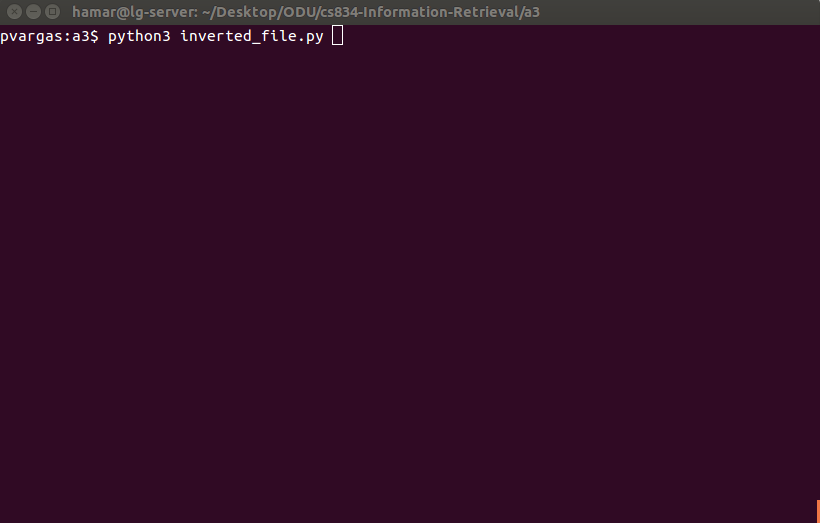
\includegraphics[scale=.40]{images/inverted-file.png}
\end{center}
\end{figure}

A document root where the collection is located is passed to generate a file (\textit{file-path.txt}) containing all resources in the collection.  The file will be used later on as a document index for the collection. The unigram index was sorted by typing unix command:\\

$\#\ $\textbf{sort zipf\_la-s.txt $>$ sorted-collection.txt}\\

The new file \textbf{sorted-collection.txt} vocabulary is indexed in alphabetical order. The sorted-collection file was uploaded as a list object in memory, and passed as a parameter to generate the index (see Listing \ref{listing:inverted-file} line 30). 

\begin{figure}[h] \label{lab:sorted-collection}
\caption{Sort Unigram}
\begin{center}
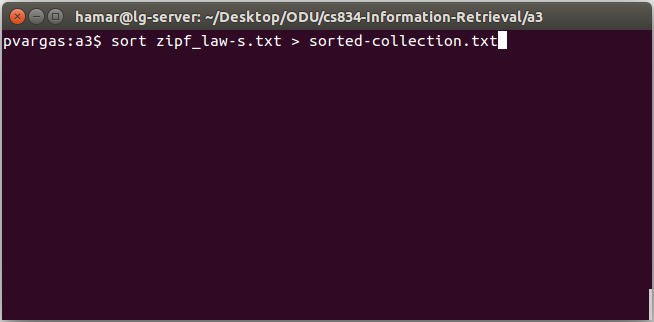
\includegraphics[scale=.40]{images/sort-collection.png}
\end{center}
\end{figure}

The inverted file index will be generated using format \textbf{999:1}, where \textbf{999} points to the document location and \textbf{1} is the term frequency at the document level (lines 64-68). 
%--------------
%  inverted_file.py
%--------------
\lstinputlisting[language=Python,
                 style=mybox, 
                 captionpos=t,
                 caption={inverted\_file.py},
				 linerange={16-105},
				 firstnumber=16,                  
                 label=listing:inverted-file,
                 ]
{../inverted_file.py}


To identify the first 1,000 words (in alphabetical order), we developed \textbf{stemmer.py}. Its main purpose is to filter non-English words from the collection. 

%--------------
%  stemmer.py
%--------------
\lstinputlisting[language=Python,
                 style=mybox, 
                 captionpos=t,
                 caption={stemmer.py},
				 linerange={16-105},
				 firstnumber=16,                  
                 label=listing:stemmr,
                 ]
{../stemmer.py}

\vspace{5mm}
\textbf{Stemmer.py} uses the \textbf{PyDictionary} library to find if a word is in the English dictionary. It iterates through a loop until the first 1,000 English words are verified.\\

For step(4) we developed \textbf{cluster.py} to generate the Dice's coefficient between all pairs of stems. We imported the library \textit{Stemmer} to stem our 1,000 word collection. The 1,000 words were loaded in memory (see Listing \ref{listing:cluster}).

\lstinputlisting[language=Python,
                 style=mybox, 
                 captionpos=t,
                 caption={cluster.py},
				 linerange={16-101},
				 firstnumber=16,                  
                 label=listing:cluster,
                 ]
{../cluster.py}

The script generates a file, clustering words with equal stem. To calculate the coefficient between pairs we generate:

\begin{equation*}
	\sum_{i=1}^{n-1}i
\end{equation*}
iterations, since we have a double loop from $i \to n$ outside $i+1 \to n$. See Listing \ref{listing:cluster} lines 70-101. Inside this double loop, we pair all possible combinations of words clustered with similar stem and calculate the Dice's coefficient by considering the documents where the pair intercept. Since we have the information from the index file, we can extract the term frequency from the document and make our calculation:

\begin{equation*}
	\frac{\medn_{ab}}{\medn_a \cdot \medn_b}
\end{equation*}
A cluster sample with Dice's coefficient is shown below:\\

\subsection{Solution}
\vspace{5mm}
/air, aire, aired, aires, airing, airings, airs
\begin{table}[h] \label{tab:dice-coef}
\begin{center}
\caption{Cluster by Stem: air}
\begin{tabular}{c | c}
\toprule
Pair & Dice's Coef\\
\toprule
(air, aire) & 0.0116\\
(air, aired) & 0.1022\\
(air, aires) & 0.0166\\
(air, airing) & 0.0399\\
(air, airings) & 0.0118\\
(air, airs) & 0.0676\\
(aire, aired) & 0.0000\\
(aire, aires) & 0.0000\\
(aire, airing) & 0.0000\\
(aire, airings) & 0.0000\\
(aire, airs) & 0.0000\\
(aired, aires) & 0.0190\\
(aired, airing) & 0.1702\\
(aired, airings) & 0.0488\\
(aired, airs) & 0.1633\\
(aires, airing) & 0.0000\\
(aires, airings) & 0.0000\\
(aires, airs) & 0.0000\\
(airing, airings) & 0.1818\\
(airing, airs) & 0.1579\\
(airings, airs) & 0.0769\\
\bottomrule
\end{tabular}
\end{center}
\end{table}

Using a threshold of 0.1500 we can re-cluster to:\\

/air, aired\\
/aired, airing, airs\\
/airing, airings, airs\\


\end{homeworkProblem}
%----------------------------------------------------------------------------------------
%	Problem 2
%----------------------------------------------------------------------------------------
\begin{homeworkProblem}[Exercise 6.2]% Custom section title
\vspace*{10pt} % Question 
Create a simple spelling corrector based on the noisy channel model. Use a
single-word language model, and an error model where all errors with the same
edit distance have the same probability. Only consider edit distances of 1 or 2.
Implement your own edit distance calculator (example code can easily be found
on the Web).

\subsection{Approach}
Our approach is based on the probability distribution model $P(w)$. The probability of a given word will be obtained from the small wikipedia collection and term frequency already generated on the previous assignment. The file \textit{zipf\_law-s.txt} was used to make the probability comparison among words.\\

A list object was used to upload the dictionary in memory (lines 98-100 Listing \ref{listing:spell-checker}). Four misspelled words were placed in an array to test our algorithm (line 26).\\

Since the entire collection consists of over 240,000 words before the distance calculation is performed, we only considered words in which length had a delta of 2 or less (lines 37-40). We passed the misspelled word and filtered dictionary to get the distance calculation (line 44).\\

In order to reduce the list size we placed each string of the list in a set to filter the words with similar number of letters. For example, if the misspelled word is \textit{teh}, the set for this word will be \{'e', 'h', 't'\} a comparison with the correct word \textit{the} will result with the same set \{'e', 'h', 't'\}. We do a subtraction between the misspelled word and the terms in the filter array. Only the words with a distance less or equal to the max distance allowed will be considered (lines 66-72). \\

Using this approach does not guarantee the words are going to be considered in equal sequence. In other words, when making a set comparison, the order of the strings are irrelevant.  The accomplished task was to ensure the number of characters between two words are within our threshold. Finally, to calculate the distance, we count the number of characters that have similar sequence with the misspelled word. An array containing a very small list is returned to calculate their probabilities (lines 74-90).\\

Finally, if $P(w/w_p) > P(e/w)$ then we will select \textit{w}. From the remaining short list, we compare all their probabilities and select the word with the highest probability (lines 46-56). 

\lstinputlisting[language=Python,
                 style=mybox, 
                 captionpos=t,
                 caption={spell-checker.py},
				 linerange={24-92},
				 firstnumber=24,                  
                 label=listing:spell-checker,
                 ]
{../spell-cheker.py}

\subsection{Solution}
Executing the program produced the following results:\\

\begin{verbatim}
Starting Time: Thu,  Nov 10, 2016 at 22:26:46
[('the', 2), ('teeth', 3)]
For Teh the correct spelling is --> the
[('the', 1), ('user', 3), ('ouse', 4)]
For couse the correct spelling is --> ouse
[('recent', 2), ('terms', 3), ('report', 4), ('tremor', 6)]
For tremmor the correct spelling is --> tremor
[('under', 1), ('contents', 3), ('street', 4), ('students', 6)]
For stodent the correct spelling is --> students

End Time:  Thu,  Nov 10, 2016 at 22:26:48
Execution Time: 2.00 seconds

Process finished with exit code 0
\end{verbatim}
\end{homeworkProblem}
%----------------------------------------------------------------------------------------
%	Problem 3
%----------------------------------------------------------------------------------------
\begin{homeworkProblem}[Exercise 6.5]% Custom section title
\vspace*{10pt} % Question 
Describe the snippet generation algorithm in Galago. Would this algorithm
work well for pages with little text content? Describe in detail how you would
modify the algorithm to improve it.\\

\subsection{Background}
The Galago snippet generation algorithm is related to the concept of relevance feedback. If a user makes a query, it will be important to know if the document we are about to retrieve is relevant to that query. So, the snippet must be a summary of the document in relation to our query.\\

Galago snippet algorithm derives from the work Luhn in the 1950s. Luhn explored the concept of ranking and selecting the top sentences in a document using a \textit{significant factor}. In order to accomplish this, we have to find which are the significant words in the document. He used the concept of word frequency as an indicator of how significant the words were for the document.\\

\begin{center}
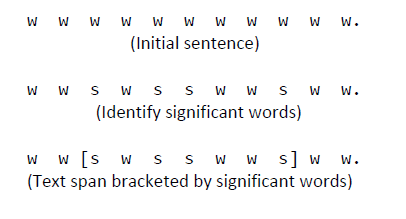
\includegraphics[scale=.75]{images/significant-words.png}
\end{center}

\subsection{Algorithm}

The code for generating \textbf{galago} query snippets was found in the \textbf{Lemur Project} at \url{https://sourceforge.net/p/lemur/galago/ci/c15406935ce7e697d7a8d0ce329606f100276921/tree/core/src/main/java/org/lemurproject/galago/core/index/corpus/SnippetGenerator.java#l11}\\

The code was written in Java. Below are some portions of the code:

\begin{verbatim}
    // Goals:  1. find as many terms as possible
    //         2. find terms that are close together
    //         3. break on sentences when possible (?)
    // BUGBUG: might not have all the terms highlighted here
    public ArrayList<SnippetRegion> combineRegions(final ArrayList<SnippetRegion> regions) {
        ArrayList<SnippetRegion> finalRegions = new ArrayList();
        SnippetRegion last = null;
        int snippetSize = 0;
        int maxSize = 40;

        for (int i = 0; i < regions.size(); i++) {
            SnippetRegion current = regions.get(i);

            if (last == null) {
                last = current;
            } else if (last.overlap(current)) {
                SnippetRegion bigger = last.merge(current);

                if (bigger.size() + snippetSize > maxSize) {
                    finalRegions.add(last);
                    last = null;
                } else {
                    last = bigger;
                }
            } else if (last.size() + snippetSize > maxSize) {
                break;
            } else {
                finalRegions.add(last);
                snippetSize += last.size();
                last = current;
            }
        }

        if (last != null && snippetSize + last.size() < maxSize) {
            finalRegions.add(last);
        }

        return finalRegions;
    }
\end{verbatim}
Then, in summary the algorithm:
\begin{enumerate}
	\item Find as many terms as possible
	\item Find terms that are close together
	\item Break on sentences when possible
\end{enumerate}

\subsection*{Would this algorithm work well for pages with little text content?}
This algorithm will not work well with little text context because the ranking of sentences will not provide enough information to make a good comparison on what region of the document is more significant than others.  Since the base of the algorithm is ranking regions or sentences, then all sentences are going to become equal and without distinction among each other.
\end{homeworkProblem}

\subsection*{Describe in detail how you would modify the algorithm to improve it}
Since the algorithm works well with plenty text:
\begin{enumerate}
	\item We need to define a threshold where the amount of text is not enough.
	\item Stem our query terms to find other possible terms related in the text.
	\item Expand our query terms to find other possible terms related in the text.
	\item Use the stems and expansion results to generate new sentences ranking.
	\item Identify regions where the added terms are more significant.
	\item Extract and display the result.
\end{enumerate}

%----------------------------------------------------------------------------------------
%	Problem 4
%----------------------------------------------------------------------------------------
\begin{homeworkProblem}[Exercise MLN1]% Custom section title
\vspace*{10pt} % Question 
MLN1: using the small wikipedia example, choose 10 words and create stem classes as per 
the algorithm on pp. 191-192
\subsection{Approach}
We modified problem 6.1 to consider only 10 words instead of 1000. So the approach and implementation are the same.

\newpage
\subsection{Solution}

\begin{figure}[h] \label{lab:sorted-collection}
\caption{Stem Class}
\begin{center}
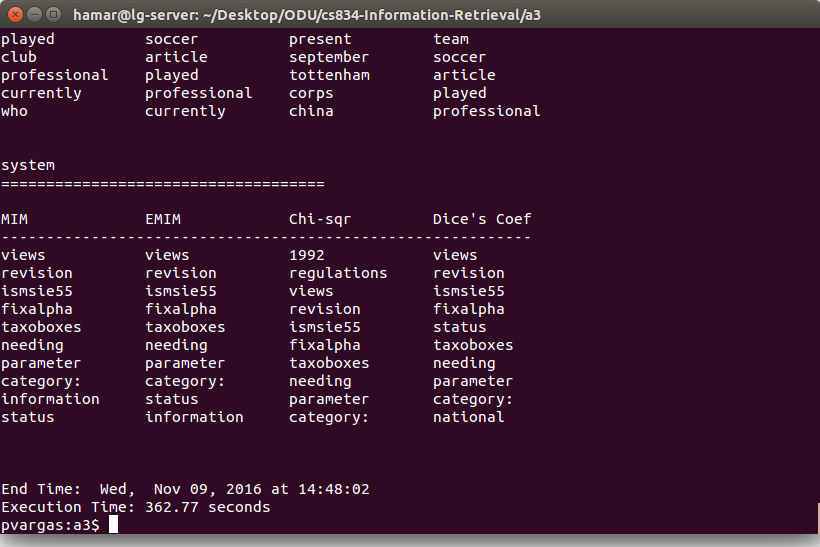
\includegraphics[scale=.40]{images/term-assoc-result.png}
\end{center}
\end{figure}


\end{homeworkProblem}
%----------------------------------------------------------------------------------------
%	Problem 5
%----------------------------------------------------------------------------------------
\begin{homeworkProblem}[Exercise MLN2]% Custom section title
\vspace*{10pt} % Question 
Using the small wikipedia example, choose 10 words and compute MIM, EMIM, chi square, 
dice association measures for full document \& 5 word windows (cf. pp. 203-205)

\subsection{Approach}
Words selected:\\

/altarpiece, resurrection, retirement, football, country, system, book, california,
department, washington

The problem was divided into three sub-problems. Each sub-problem was related to a module developed within python script \textbf{term-association.py}.\\

\begin{itemize}
	\item Getting file index.
	\item Getting file content.
	\item Obtaining term frequency.
\end{itemize}

\subsubsection{Running Script}
We can generate the term association by typing from the command prompt:\\

$\#\ $\textbf{python3 term-association.py}\\

\begin{figure}[h] \label{lab:term-assc-py}
\caption{Generating Term Association}
\begin{center}
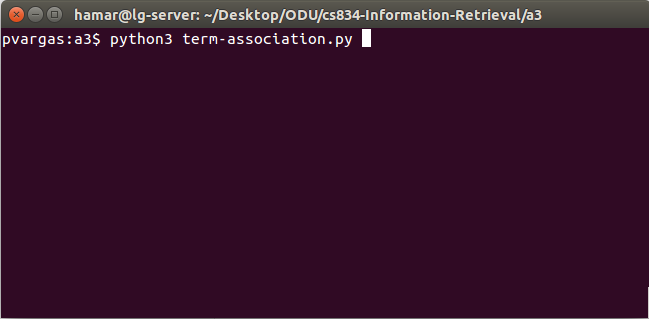
\includegraphics[scale=.40]{images/term-assoc-py.png}
\end{center}
\end{figure}

\subsubsection{Main Module}
This module directs the script to accomplish various tasks, and provide the required data prior to its execution. Since we did not remove the stop words from the index, they have to be identified and removed prior to the term association calculation, otherwise we will be certainly associating stop-words with our terms, thus providing undesired results. These stop-words in Listing \ref{listing:term-assoc-main} line 23, were obtained by inspecting our collection term frequency in file:\textit{zipf\_law.txt}. The higher frequency terms were visually inspected, copied and plugged into the list object \textbf{stop-words}. This object was used for comparison and removal of those existing words in the body of inspected documents. There were some non-stop-words added to this object that did not meet the frequency requirement to be considered stop-words, but were added because they became part of the generated index, but they were meaningless to our term association. \\

The list of terms for which are we going to find the association in the collection are loaded in a list object (\textbf{vocabulary}) in line 32. The inverted file index is loaded into memory, and as it was stated before, it has the form \textit{term} [999:\textit{freq},], where 999 refers to the document index in \textit{inverted-file.txt} and \textit{freq} is the frequency of the term at the document level.\\

The list of terms contained in \textbf{vocabulary} is inspected to ensured they are contained in our inverted file index. In case the term is not included, it will be inspected and added to the inverted file object for the collection (lines 50-52). \\

The window size (line 58) and the terms to be associated (\textbf{vocabulary}) are passed as a parameter (lines 58-59) to find and measure all the terms within the window proximity of the terms. An object (\textbf{term\_data}) is returned containing the frequency of words associated to \textbf{vocabulary} at the document level. This information will be used (line 61) to calculate the association using various measures: \textit{MIM, EMIM, Chi-square} and \textit{Dice's coefficient}.\\

\lstinputlisting[language=Python,
                 style=mybox, 
                 captionpos=t,
                 caption={term-association.py - main module},
				 linerange={20-93},
				 firstnumber=20,                  
                 label=listing:term-assoc-main,
                 ]
{../term-association.py}

Finally, the values provided from the different measures are sorted in descending order (line 63-91) to display the $k=10$ words strongly associated with a particular methodology.

\subsubsection{Getting file index}
This module generates the index of any term in the parameter list that was not included in the inverted file. The parameter list is an array of terms by which its association measure will be calculated (\textbf{vocabulary}). An iteration is performed on all the resources in our collection to inspect its content. The document index is stored in \textbf{file\_no} (line 132) and increased by one every time a new document gets inspected. \\

The document contents are extracted from module \textit{get\_file\_content()} (line 135) and the frequency of all the terms within the document are obtained using the python library \textbf{Counter} (line 138).

\lstinputlisting[language=Python,
                 style=mybox, 
                 captionpos=t,
                 caption={term-association.py - build index module},
				 linerange={128-146},
				 firstnumber=128,                  
                 label=listing:term-assoc-build-idx,
                 ]
{../term-association.py}

\vspace{5mm}
Finally, if a term in \textbf{vocabulary} is found inside the document, then it is added to the index using format \textit{term} [999:\textit{freq}]. See lines 141-144.

\subsubsection{Getting file content}
Since this functionally is commonly used to solve our main problem, in order to maintain consistency and repeated work, a module was created to extract the content of a particular web-page resource. The module takes as a parameter the location where the resource is stored, reads the file and removes all the contents of no interest such as [,= etc. The return value is an array containing all terms within the document.\\

\lstinputlisting[language=Python,
                 style=mybox, 
                 captionpos=t,
                 caption={term-association.py - get content module},
				 linerange={237-249},
				 firstnumber=237,                  
                 label=listing:term-assoc-get-content,
                 ]
{../term-association.py}

\subsubsection{Obtaining terms frequencies}
The meat of our solution resides within this module. The main scope is to pair a document with a term or list of terms. Then, for each term, find the location (index) where the term is positioned within the document. By inspecting a window size \textit{w} to the left and right of the current position, we can record the words with proximity \textit{w} to our term. The last step is to find out the frequency of those words within proximity \textit{w} to our term within the document. The process is repeated for all the documents in the collection. The resulting object is a dictionary of dictionaries containing a term and their words with proximity \textit{w} to their frequency:\\

\begin{center}
	\{\textit{term}: \{\textit{word1:freq}, \textit{word2:freq}, $\cdots$ \}\}
\end{center}

The list of terms (\textbf{vocabulary}) for which we are going to measure their association and the \textit{window} size is passed as parameter to this module. The inverted file provides the resources where these terms are located. For every document where a term is found in the collection (Listing \ref{listing:term-assoc-get-term-freq} line 154), we can find the frequency of the term by splitting data value [999:\textit{freq}] and obtaining the left side of the colon (':') or the pointer to the resource (line 155).\\

The content of the file is stored in the list object \textbf{data} (line 157), then all the stop-words are remove from \textbf{data} (lines 160-166). The frequency of words in \textbf{data} can be found using library \textit{Counter}, the result is stored into dictionary object \textbf{counts} (line 168).\\

Then, we proceed to find the first position where the \textit{term} is located within \textbf{data} object (line 171). First, we get \textit{window} number of words to the left of our current position (lines 175-179) taking in consideration that a number of words could point \textit{n} positions before the beginning of \textbf{data} array. Then, we do the same going to the right of our current \textit{term} position taking in consideration that a number of words could point \textit{n} positions beyond the end of \textbf{data} array (lines 181-187).\\

To make a distinction between the frequency that a word appears within the document and the frequency a word appears within a \textit{window} with a \textit{term} in the document the '\_' character was added to the dictionary to indicate this distinction. This frequency calculation is performed in lines 189-203 Listing \ref{listing:term-assoc-get-term-freq}.\\

Since, it is possible that a \textit{term} could be found more than once with in a document we have to find the next position where the \textit{term} is located in \textbf{data} object. We will continue this process until no more \textit{terms} are found in the object (lines 206-232).  Finally, the result is a dictionary of dictionary (\textbf{window\_term}) in line 234.\\

\lstinputlisting[language=Python,
                 style=mybox, 
                 captionpos=t,
                 caption={term-association.py - Get Term Frequency Module},
				 linerange={149-234},
				 firstnumber=149,                  
                 label=listing:term-assoc-get-term-freq
                 ]
{../term-association.py}

\subsection{Solution}
\import{./}{table-p5.tex}

\newpage
The association measure seems to work remarkable well. If we take a look at the terms associated with the word 'washington' on Table \ref{tab:washington} we can see that using the Mutual Information measure (\textit{MIM}), \textbf{Washington} is associated with the ``Washington Post'', ``West Washington'', ``Washington school'', ``Washington DC''. The \textit{EMIM} measure is very similar to the \textit{MIM}, but in different ranking order.\\

The Chi-square for the same term seems to be more related with sports words related to the word \textbf{Washington}, such as fox, nfl, games, jets, etc. There is also a good association with the word \textbf{Washington} using the \textit{Dice's coefficient}\\
\end{homeworkProblem}
%----------------------------------------------------------------------------------------
%	Bibliography
%----------------------------------------------------------------------------------------
\newpage
\bibliography{bibliography}
\bibliographystyle{siam}
%\begin{thebibliography}{9}
%\bibitem{Lutz} 
%Lutz, Mark (2013). List and Dictionaries. \textit{Learning Python} (5th ed.). (pp. %262-263). Sebastopol, CA: O'Reilly Media.
%
%\bibitem{ci}
%Segarn, Toby. Programming Collective Intelligence. \textit{Building Smart Web 2.0 Application}. (pp 29-53). Sebastopol, CA: O'Reilly Media.

%\bibitem{sitemaps}
%Sitemaps Schema. (n.d.) Retrieved September 21, 2016, from \url{http://www.sitemaps.org/schemas/sitemap/0.9}

%\end{thebibliography}
\end{document}

